\chapter{Wearable Edge AI}
\label{chap:wearable-edge-ai}

\nomenclature{CPU}{Central Processing Unit}
\nomenclature{PCB}{Printed Circuit Board}
\nomenclature{WBAN}{Wireless Body-Area Network}

\begin{figure}[h!]
    \centering
    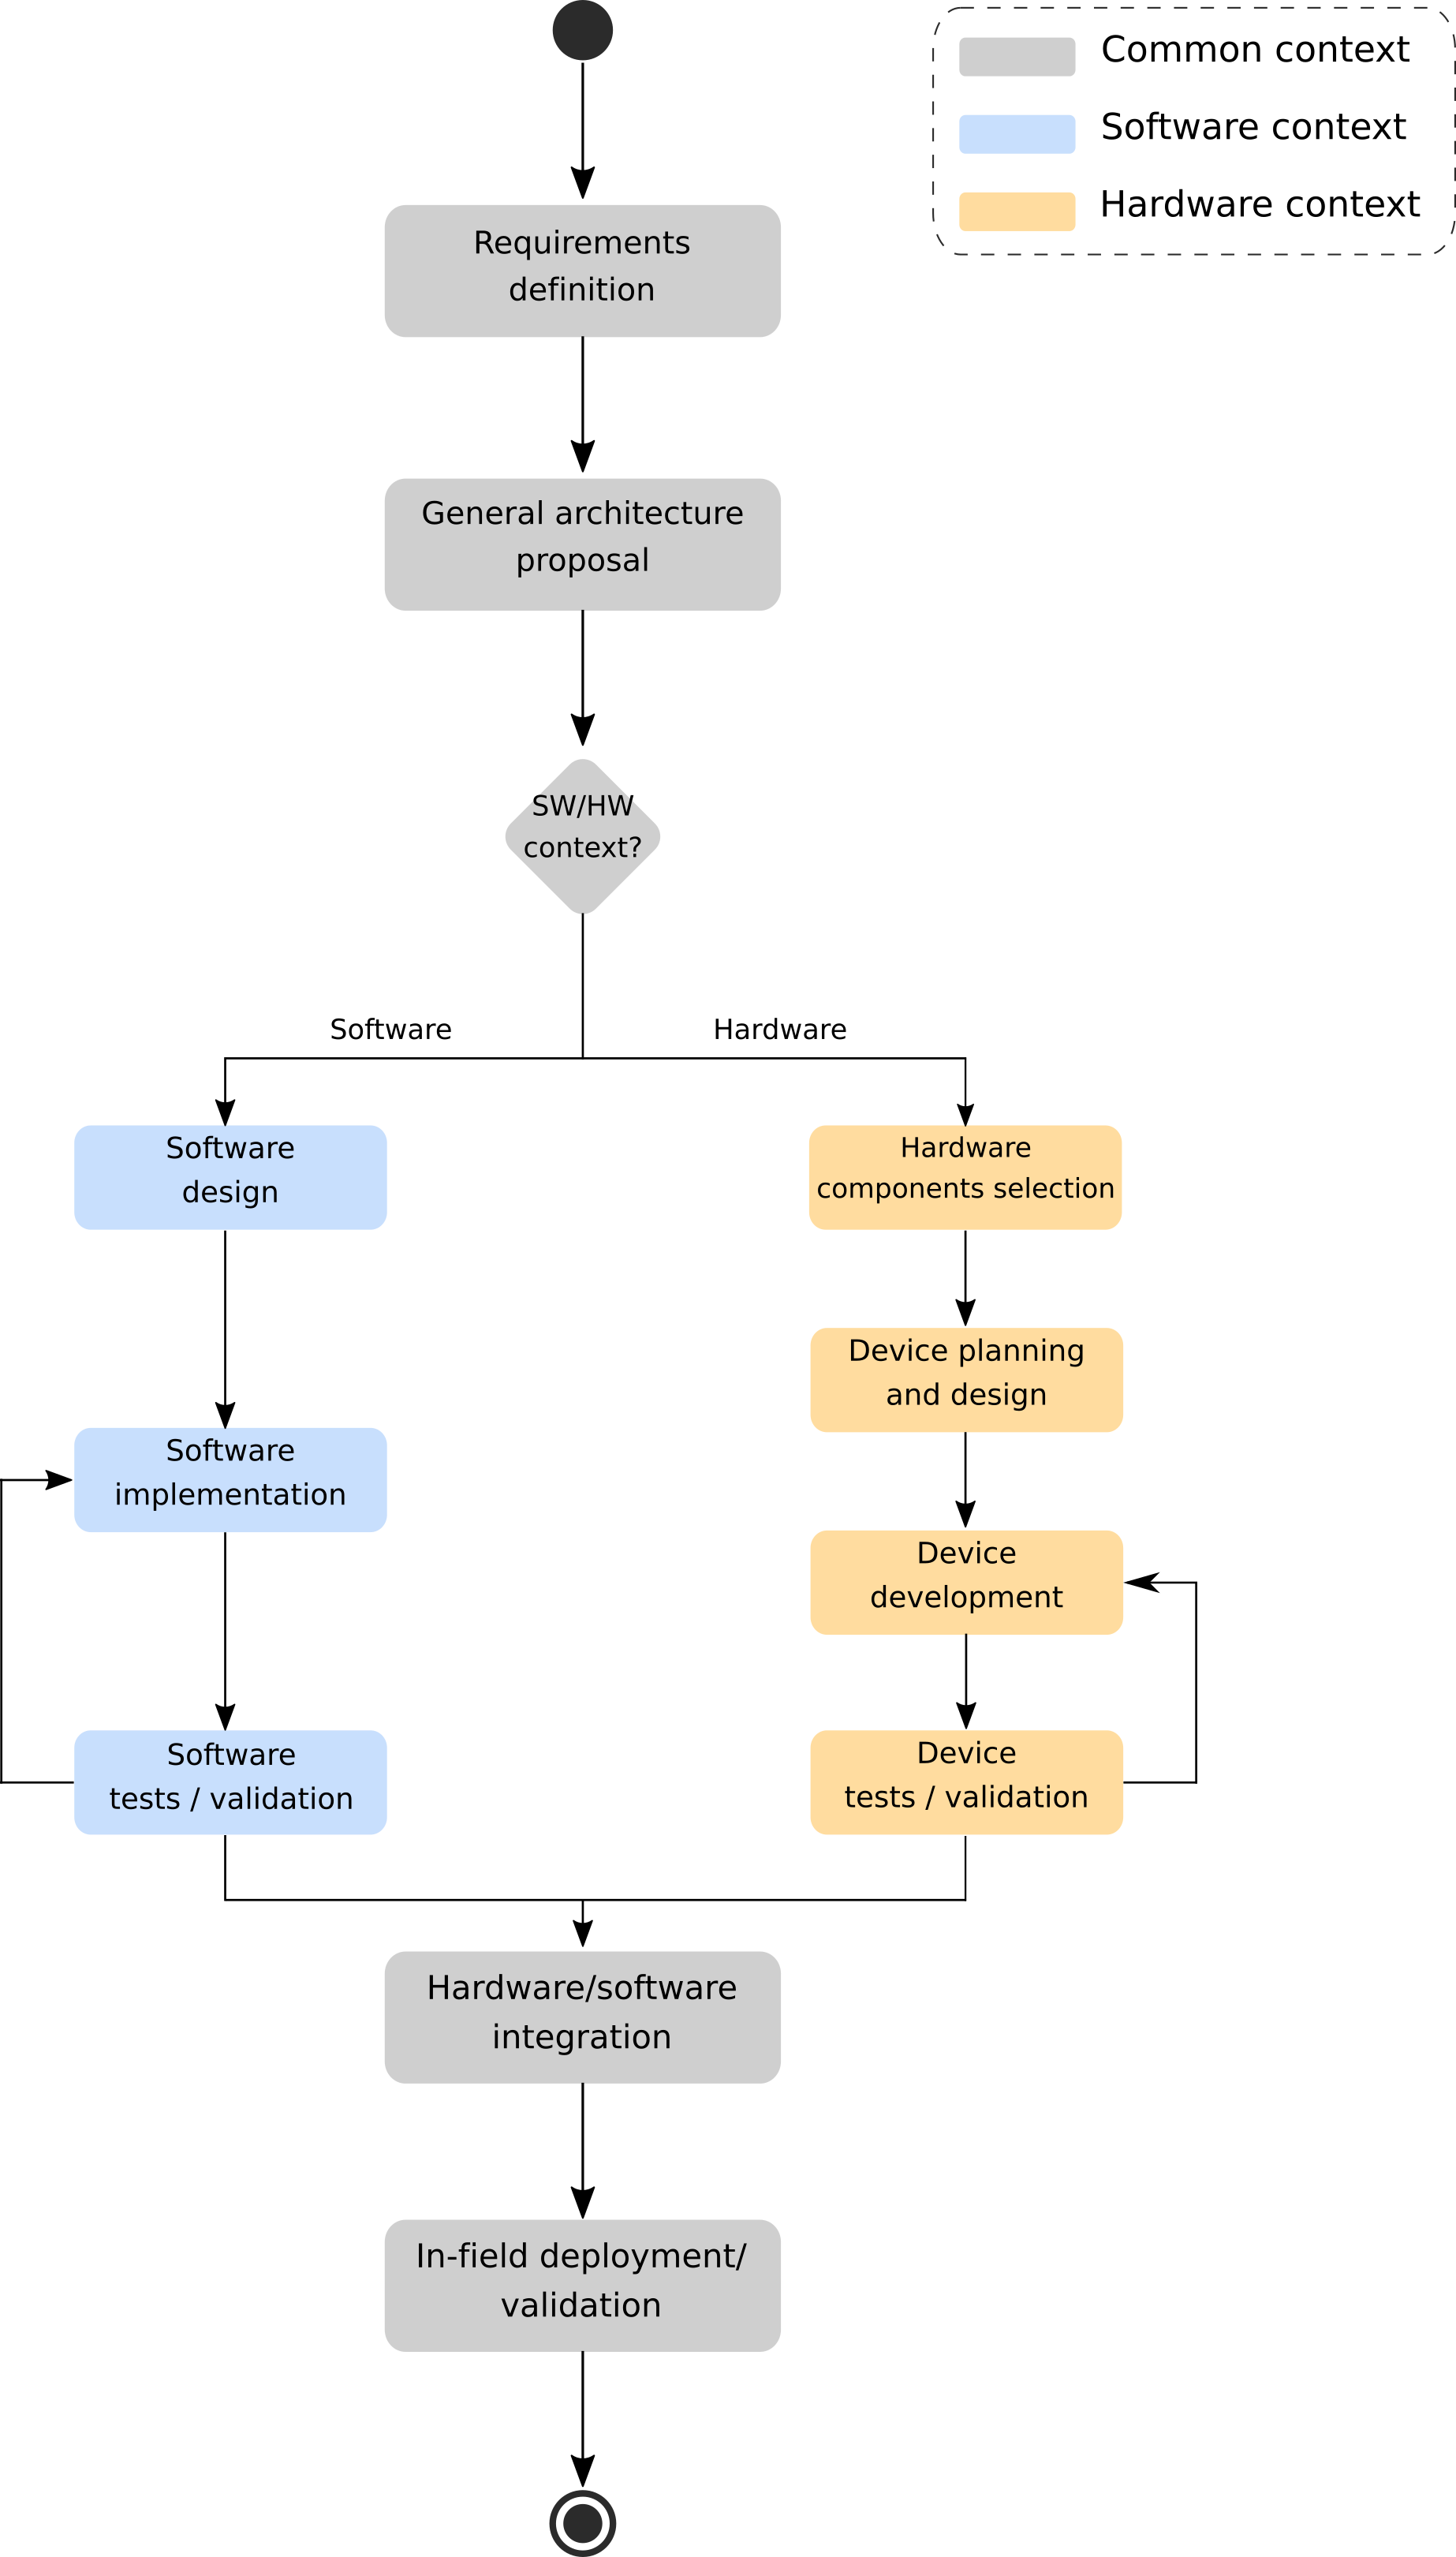
\includegraphics[width = .5\linewidth]{Figures/design_diagram.png}
    \caption{Original Hardware and Software co-design process, presented in \cite{silva2019field}}
    \label{fig:hw-sw-codesign}
\end{figure}

This chapter discusses the creation of the \textit{Wearable Edge AI} concept. Our discussion begins with an understanding of how cooperative wearable systems work. Then, we review the hardware/software co-design process. Finally, we assess the wearable edge AI concept, surrounding its constraints and its creation and validation processes.

Our concept starts from the wearable systems perspective. Thus, it is required to understand the design process behind them. As an inheritance from their embedded systems' origin, wearable devices and systems usually follow a process known as hardware and software co-design \cite{silva2019field}, exemplified in Figure \ref{fig:hw-sw-codesign}. 

As displayed, a series of steps are required to produce these solutions. Initially, there are two general steps to start projecting these appliances:

\begin{itemize}
    \item \textbf{Requirements definition:} This stage involves collecting, assessing, and examining the system requirements. This is achieved by conducting a thorough analysis of the stakeholders' needs;
    
    \item \textbf{General architecture proposal:} During this stage, professionals utilize the data collected from the previous step to create a preliminary outline of the proposal. This initial blueprint necessitates defining the limitations for both software and hardware to strategize the flow of information.
\end{itemize}

Following these preliminary stages, there are several simultaneous activities related to the software and hardware characteristics. These steps occur concurrently since their outcomes are interdependent. They are:

\begin{itemize}
    \item \textbf{Hardware:} 
    \begin{itemize}
        \item \textbf{Hardware components selection:} The initial step in the hardware phase is to list the necessary hardware components required to execute the proposed tasks and functions.
        \item \textbf{Prototype planning and design:} Hardware components act as input data for devising and developing the final prototype. During this stage, connections between components are specified, and if required, the Printed Circuit Board (PCB) layout is outlined;
        \item \textbf{Prototype development:} This phase involves the production of the wearable device. The primary Central Processing Unit (CPU) and hardware peripheral components are physically linked, potentially employing the final version of the PCBs created in the previous stage. Finally, the components can be attached to the garment;
        \item \textbf{Device tests/validation:} Multiple rounds of on-site hardware testing and validation are conducted to authenticate the connections established with each component. If any issues arise during this stage, they can be rectified or altered in a new development round.
    \end{itemize}
    \item \textbf{Software:}
    \begin{itemize}
        \item \textbf{Software design:} The previously stated requirements can also serve as a guide for devising the relevant software. This phase entails defining functionalities and how internal modules will communicate with one another;
        \item \textbf{Software implementation:} The design created earlier can now be utilized as a point of reference for precisely coding the software. Typically, specific and lightweight programming languages/frameworks can be employed during this stage, depending on the requirements of the entire solution;
        \item \textbf{Software tests/validation:} This module is responsible for testing and verifying whether the resultant software adheres to the previously stated requirements. If the solution fails to meet the necessary requirements or does not pass the validation tests, a new development round can be initiated.
    \end{itemize}
\end{itemize}

The remaining blocks are used by both contexts:

\begin{itemize}
    \item \textbf{Hardware/software integration:} This stage involves integrating the previously developed hardware and software components. This is a crucial step since both sections were separately developed until this point. Basic and complex functionalities can be assessed to determine whether they produce the desired output.
    
    \item \textbf{In-field deployment/validation:} This marks the final stage in the design of wearable systems. The wearable device, which now incorporates integrated hardware and software modules, is deployed and authenticated through field sessions. This moment is also utilized in numerous research projects to collect and retrieve empirical data. 
\end{itemize}

\section{Cooperative Wearable Systems}

The \textit{Wearable Edge AI} concept originates from the recognition that wearable systems do not function as isolated processing units. In Chapter \ref{chap:intro}, we highlighted that Wearable Computing systems can be incorporated into cyber-physical applications.

Augimeri et al. \cite{augimeri2011collaborative} and Fortino et al. \cite{fortino2015framework} present four distinct propositions for collaborative body sensors. In two of these propositions, data collected from a single user provides information to one or several stations. In the other two, data collected from multiple users is utilized to feed one or several stations. Similarly, to comprehend the methods of collaborating using wearable devices, we categorize Cooperative Wearable Systems into two scenarios:

\begin{enumerate}
    \item Single-User Cooperative Wearable Systems,
    \item Multiple-User Cooperative Wearable Systems.
\end{enumerate}

The first type happens when the same user utilizes multiple wearable devices to compose a system, feeding one or multiple applications in base stations. The second type occurs when many users wear the same equipment, with post-processed data and flexibility gained in the final appliances in individual or various consumer stations.

\subsubsection{Single-User Cooperative Wearable Systems}

Wearable compositions are crucial for monitoring both the user and the context of the environment. Mihovska and Sarkar \cite{mihovska2018cooperative} introduce a vital concept for this context: Human-Centric Sensing. According to these researchers, the Internet of Things (IoT) and connectivity of modern devices provide the necessary tools to establish cooperative systems around the user. These systems can monitor both user signals and the surrounding environment.

Zhang et al. \cite{zhang2019cooperative} proposed a cooperative environment based on a glove-shaped pressure sensor and an armband to enable gesture recognition for Human-Computer Interaction devices. They conducted a series of tests to verify the recognition accuracy of their system.

Peng and Peng \cite{peng2016cooperative} assert that Body-Area Networks have become a critical tool for creating innovative healthcare solutions using collaborative wearable devices. They proposed a cooperative communication strategy to integrate multiple devices in a Wireless Body-Area Network (WBAN) and validated their proposal through simulations.

Nguyen-Huu et al. \cite{nguyen2018smartwatch} present a combination of a wearable device and smartphone working together to monitor daily activities in an indoor environment. Their system utilizes both an armband and a smartphone to gather sensor data, process and recognize activities, and transmit this information to a web server for further analysis. They validated their system through performance evaluations on their activity recognition and lifelogging algorithms.

Most of the proposed systems and architectures employ wearable devices as IoT nodes in a Wireless Body-Area Network, and in some instances, smartphones serve as connection gateways. Finally, these works follow the same systematic process, beginning with requirement analysis, architecture proposal, implementation, and validation.

\subsubsection{Multiple-User Cooperative Wearable Systems}
\label{subsec: MUCWS}

Pimentel et al. \cite{pimentel2019wearable} developed a system that monitors the stress levels of multiple surgeons by using commercial wearable devices for vital signs monitoring, such as ECG and actigraphy signals. The data gathered from these devices is sent to an Android application that marks events, creates reports, and stores the data in a database. The authors validated their proposal by conducting statistical studies on the self-assessment tools present in the Android application.

In another study, Prakash and Ganesh \cite{prakash2016establishment} established a communication environment for cooperative health monitoring in hospitals using wearable devices. They tested their proposal using network simulator applications to verify the packet transmission performance.

Pham et al. \cite{pham2018validation} proposed a wearable-based system environment to monitor older adults and patients with Parkinson's disease. Their architecture was based on IoT wearable devices with Inertial Measurement Units (IMUs) located on the user's lower limb. To validate their proposal, they tested their environment and system with actual target users and compared the results with video recognition using statistical analysis. These studies followed a similar systematic process, including analyzing the context of use and system requirements, proposing an architecture, assembling a prototype environment, and performing validation tests.

Even in a multi-user context, the current state-of-the-art works follow a systematic process in proposing wearable systems. This includes analyzing the context of use and gathering system requirements, proposing an architecture, assembling a prototype environment to test the proposal, and performing validation tests.

\section{Wearable Edge AI}

Field research environments usually lack the infrastructure required to integrate Edge wearable devices with computer systems. Wearable Edge AI is a concept that aims to provide services to ecological researchers and practitioners by offering local services based on artificial intelligence applications. The concept enables embedded devices to perform machine learning models that assist humans in the decision-making process in real-time.

The growing interest in machine learning, deep learning, and other computational intelligence applications has led to discussions on how to bring these algorithms to the edge. According to Chen and Ran \cite{chen2019deep}, the main challenges of using machine and deep learning in this context are latency, scalability, and privacy. These technologies are typically used for Computer Vision and Natural Language Processing, and relevant features in these applications include cost, reliability, latency, and privacy, as stated by Wang et al. \cite{wang2020convergence}.
 
An increasing number of wearable computing applications use edge computing to provide insights based on machine learning. For instance, there are appliances in health monitoring \cite{manogaran2019wearable,uddin2019wearable,liu2018cooperative}, ergonomics \cite{vega2019p}, activity tracking \cite{kumari2017wearable}, and so on. Most of these applications are user-centered and focus on monitoring the users' conditions rather than the environment. Although there are many applications and common features, the authors have yet to define Wearable Edge AI as a single topic. Therefore, this work aims to formalize the constraints and design patterns for such applications.

Considering these aspects, we produced an entry for the Wearable Edge AI concept. It considers the aspects raised in this chapter and Chapter \ref{chap:establishing} as foundations. We define Wearable Edge AI as:

\begin{itemize}
	\item Wearable Edge AI is the set of methods that describes the design process and validation of solutions that combine wearable computing, edge computing, and machine learning concepts in developing novel appliances, systems, and applications to solve real-world problems.
\end{itemize}

Although this concept is very similar to the one presented in Chapter \ref{chap:establishing}, the presence of wearable computing concepts and constraints is a crucial difference. Wearable applications have constraints that are not included in edge computing by itself. These devices are especially constrained in resources and capabilities, reduced in size, but require the usage of machine and deep learning algorithms to perform inferences.

\subsection{Rethinking the hardware/software co-design for Edge AI solutions}
 
The co-design principle of hardware and software is crucial while designing new solutions for embedded and wearable systems \cite{demicheli2013hardware,de1997hardware}. This principle guides the process of designing and validating parallel hardware and software aspects, which later integrate into novel systems.
 
However, in this text, we suggest a new approach to this pattern. We believe that architectural factors must also be validated parallelly during the design process in edge computing and IoT approaches. To illustrate this, Figure \ref{fig:codesign-all} displays the traditional and new diagrams for the co-design. While Figure \ref{fig:codesign-1.0} shows the traditional approach for the Hardware/Software (HW/SW) co-design pattern, Figure \ref{fig:codesign-2.0} explores a new branch for designing and validating the architecture in parallel with hardware and software constraints.
 
\begin{figure}[ht]
\centering
\begin{subfigure}{.4\textwidth}
  \centering
  % include first image
  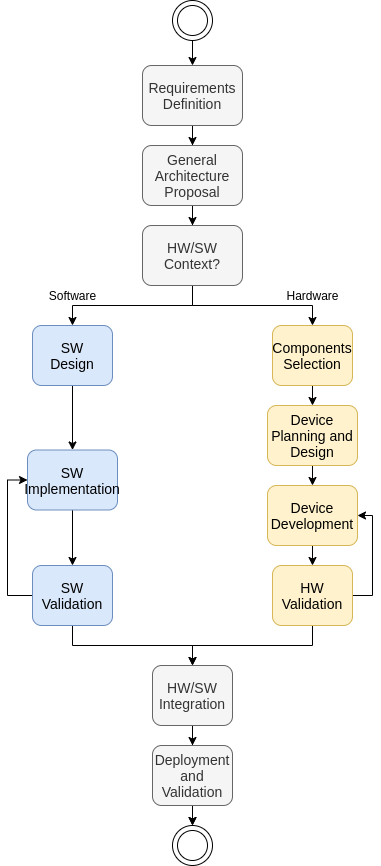
\includegraphics[width=.95\linewidth]{Figures/codesign-1.0.png}  
  \caption{Co-design considering HW/SW}
  \label{fig:codesign-1.0}
\end{subfigure}
\begin{subfigure}{.4\textwidth}
  \centering
  % include second image
  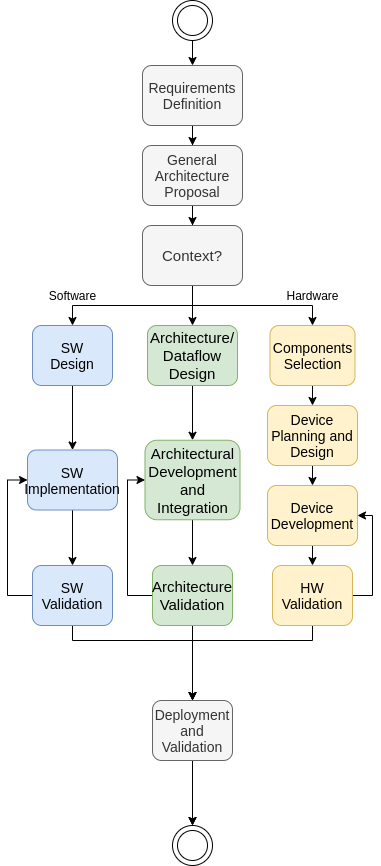
\includegraphics[width=\linewidth]{Figures/codesign-2.0.png}  
  \caption{New co-design approach}
  \label{fig:codesign-2.0}
\end{subfigure}
\caption{Co-design principle diagrams. The traditional approach does not consider architectural aspects in parallel with the HW and SW design.}
\label{fig:codesign-all}
\end{figure}

The traditional co-design approach typically begins with defining requirements and proposing a general architecture. Then, the constraints are segregated between hardware and software contexts, and the development of both aspects proceeds in parallel. After validating both components, the solution is integrated. This architecture is effective for designing single solutions for wearable and embedded systems, regardless of their abstraction levels. However, when dealing with multiple and variable architectures, this approach becomes fragile. If the validation after integration fails due to architectural traits, the solution becomes obsolete. This problem becomes even more critical when designing a Wearable Edge AI, where such factors cannot be ignored.

Thus, we suggest that architecture validation should be a new branch after context splitting. When designing new devices, identifying the essential aspects of architectural design and validating these designs during the proposal process is crucial. Finally, the integration must happen in parallel, and the last stage is deploying and validating all systems together. In the architecture branch, represented by green blocks in Figure \ref{fig:codesign-2.0}, there are three new stages:

\begin{itemize}
    \item \textit{Architecture/Dataflow Design}: In this stage, the proposal must identify how the devices communicate within the network. In the context of IoT and Edge Computing, devices communicate with each other providing services, insights, and information. Integrating devices in the same WBAN/WPAN, or even multiple devices with multiple WLAN users, requires a dataflow design.
    \item \textit{Architectural Development and Integration}: After defining the roles of each device within the network, as well as the integration protocols, the architecture must be developed in parallel with the integration of hardware components and individual software traits.
    \item \textit{Architecture Validation}: Like the other branches, the architecture must also be validated using formally-defined tests. This aspect enforces the design process and identifies flaws in the development process that must be assessed.
\end{itemize}

As displayed, these conditions help assessing the possibility of creating solutions combining the concepts of wearable computing, edge computing, and AI. We have previously studied the development of an Edge AI concept. Now, we define Wearable Edge AI as the set of methods that describes the design process and validation of solutions that combine wearable computing and Edge AI concepts in developing novel appliances, systems, and applications to solve real-world problems.

% \subsection{Hardware constraints}

% \subsection{Software constraints}

% \subsection{Architecture constraints}

\cleardoublepage